\subsection{Side Scan Sonar SLAM Architecture}
\begin{figure}[H]
    \centering
    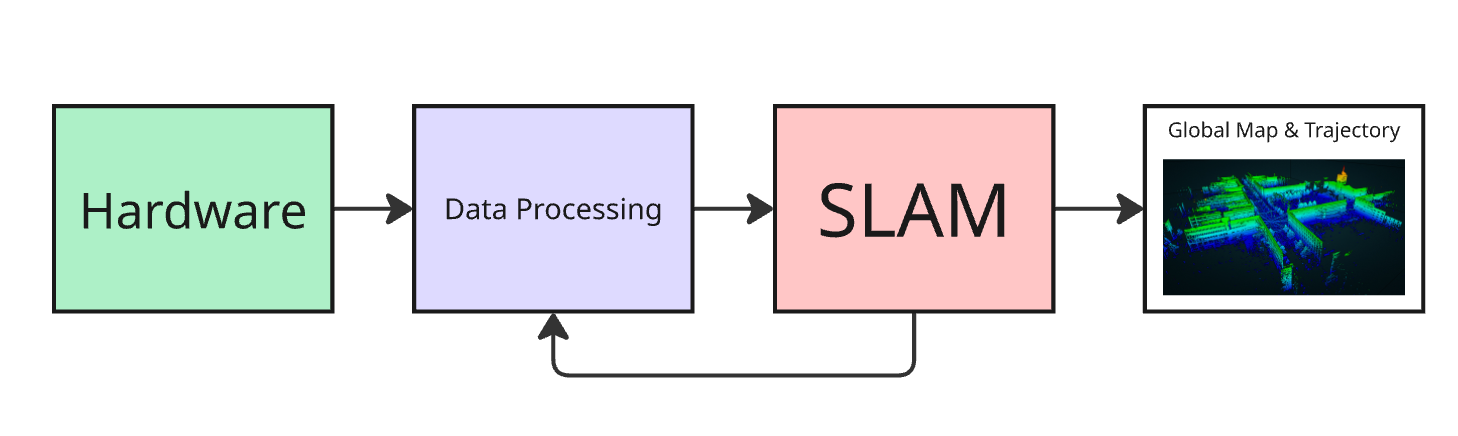
\includegraphics[width=1.0\linewidth]{Pictures/Introduction/SSS_SLAM_Architecture/Simplified.png}
    \caption{A simplified picture of SSS SLAM pipeline from raw sensor data to global map}
    \label{fig:SSS-SLAM-Architecture-Simplified}
\end{figure}
\begin{figure}[H]
    \centering
    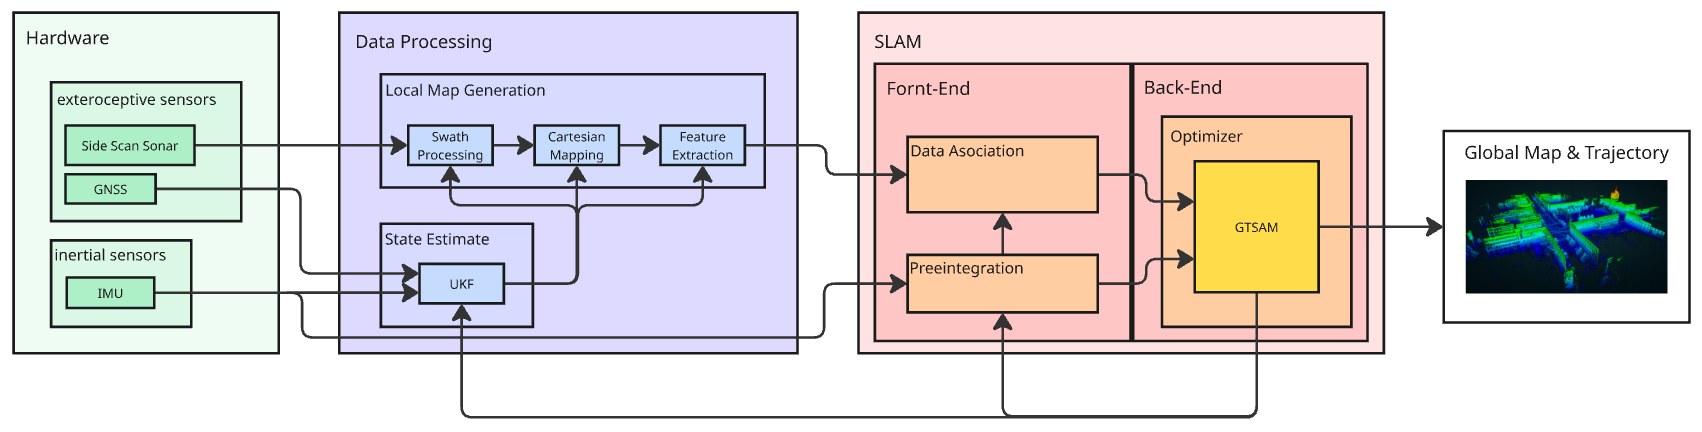
\includegraphics[width=1.0\linewidth]{Pictures/Introduction/SSS_SLAM_Architecture/Full.png}
    \caption{A picture of the whole SSS SLAM pipeline in detail from raw sensor data to global map}
    \label{fig:SSS-SLAM-Architecture-Full}
\end{figure}
\noindent
SOme images here of basic overvies
\\ \\
Talk abit on SLAM
\\ \\
Then a picture of complex overview
\\ \\
Talk a bit more in depth on slam
\\ \\
from modeling perspective IMU will be considered at center of gravity COG that will be discussing in detail the reason why in system modeling part. As well as assuming that the environment we are mapping is static or relativity static with very little change in the environment over time this again will be further elaborated on Data Association chaper. ALso mention that the architecture bases itself on Graph Based SLAM.
\\ \\
Also mention that this project will assume the enviroment that is being mapped is near static or very slowly varying. As more sufisticated Data Asociation algorithms woudl be needed to achieve mapping in highly dynamic envoroemnts. ANd the the sea bed it is a slowly varying enviroment with very litle changes over short periods of time. 